\documentclass{article}
\title{Demonstration of Preemptive numbering}
\author{BRM}
\usepackage{graphicx}
\begin{document}
\maketitle
\section{Introduction}\label{Intro}
You will see: sections \ref{First} and \ref{Second};
subsections  \ref{First.First}, \ref{First.Second},
\ref{Second.First} and \ref{Second.Second};
some equations \ref{First.Pythagoras} and \ref{Second.Einstein};
as well as some figures \ref{First.Sunset},  \ref{Second.Sunset}.

\section{First Section}\label{First}
The first section of the document.
\subsection{First Subsection}\label{First.First}
A subsection with some math.
\begin{equation}\label{First.Pythagoras}
  a^2+b^2=c^2
\end{equation}
\subsection{Second Subsection}\label{First.Second}
A subsection with a figure.
\begin{figure}
  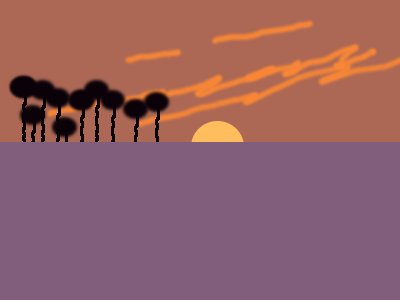
\includegraphics{sunset}
  \caption{A beautiful sunset\label{First.Sunset}}
\end{figure}
\section{Second Section}\label{Second}
The section section of the document.
\subsection{First Subsection}\label{Second.First}
Another subsection with some math.
\begin{equation}\label{Second.Einstein}
  E=mc^2
\end{equation}
\subsection{Second Subsection}\label{Second.Second}
Another subsection with a figure.
\begin{figure}
  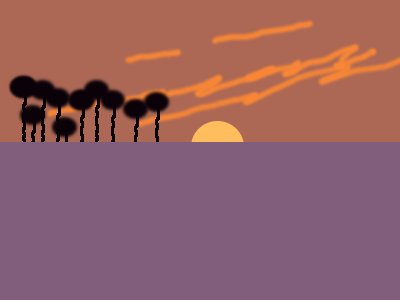
\includegraphics{sunset}
  \caption{The same beautiful sunset\label{Second.Sunset}}
\end{figure}

\end{document}